  % this file is called up by thesis.tex
% content in this file will be fed into the main document
% ----------------------- name of chapter  -------------------------
%\newgeometry{top=-0.6cm}
\chapter{Mass Resolution}
\label{appendix:mass_resolution}

% ----------------------- paths to graphics ------------------------

% change according to folder and file names
\ifpdf
    \graphicspath{Appendices/AP2/figures/}
\else
    \graphicspath{Appendices/AP2/figures/}
\fi

% ----------------------- contents from here ------------------------

\noindent The signal events are reconstructed using a $\chi^2$ minimisation as
it is described in~\cref{sec:selection}. The central value for the masses and the widths in~\cref{eq:chi2tt} are taken from the simulated FCNC \ttbar decay signal samples. 
The values are extracted from the Bukin fits~\cite{Bukin} to the masses of the top quarks and \PW boson
reconstructed by matching the true generated $q$- and $b$-quarks to the reconstructed
jets within the $\Delta R < 0.4$, assuming the missing transverse momentum to be the neutrino transverse momentum,
and setting the longitudinal momentum of the neutrino to the $p_z$ of
the true generated particle.
These represent the optimal resolution of
the reconstructed \Pqt-quarks and \PW boson masses in the FCNC \ttbar decay signal events. 
These fits are shown in \cref{fig:app-mass:bla} along with the mean values and standard
deviations.

\begin{figure}[htbp]
%		\begin{adjustwidth}{-1.4cm}{}
			\begin{tabular}{ccc}
				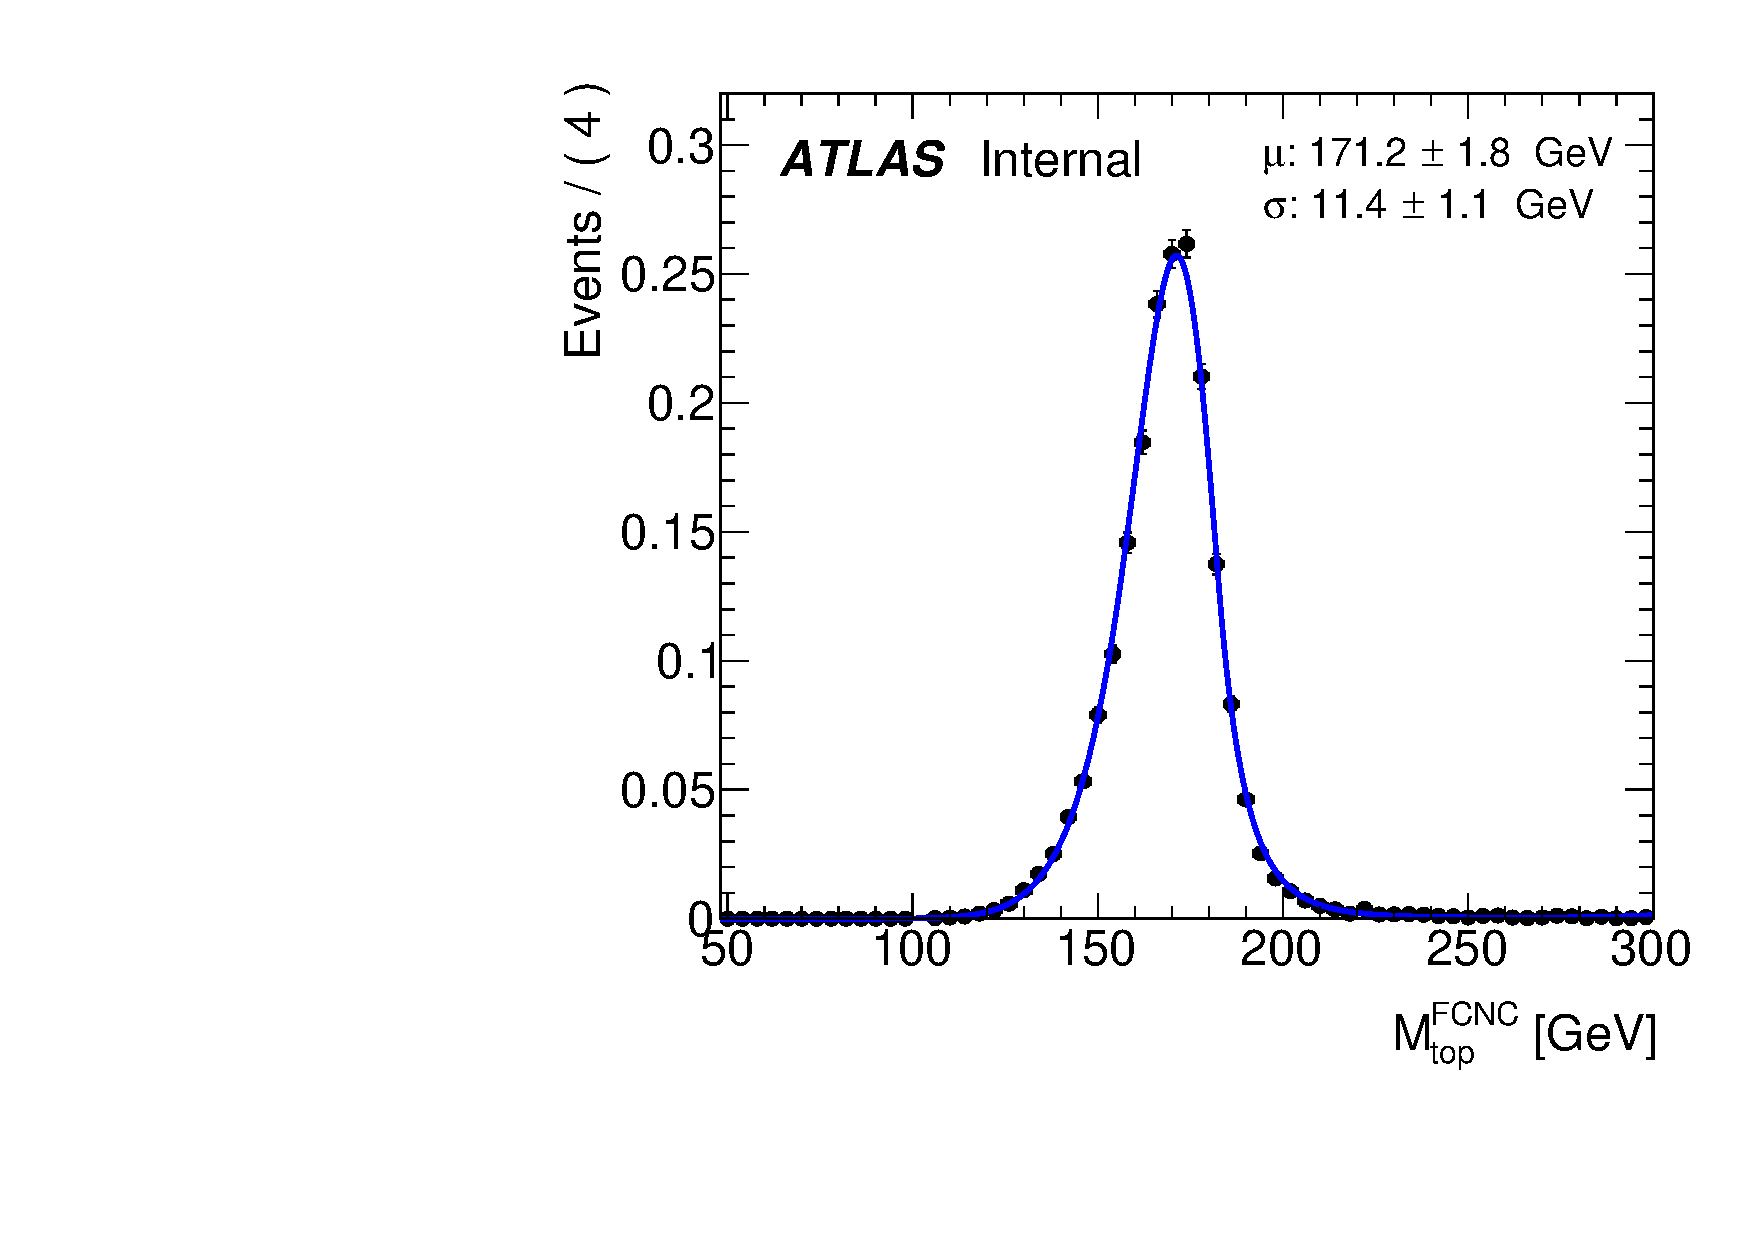
\includegraphics[width=.45\textwidth]{Appendices/AP2/figures/topFCNC} &
				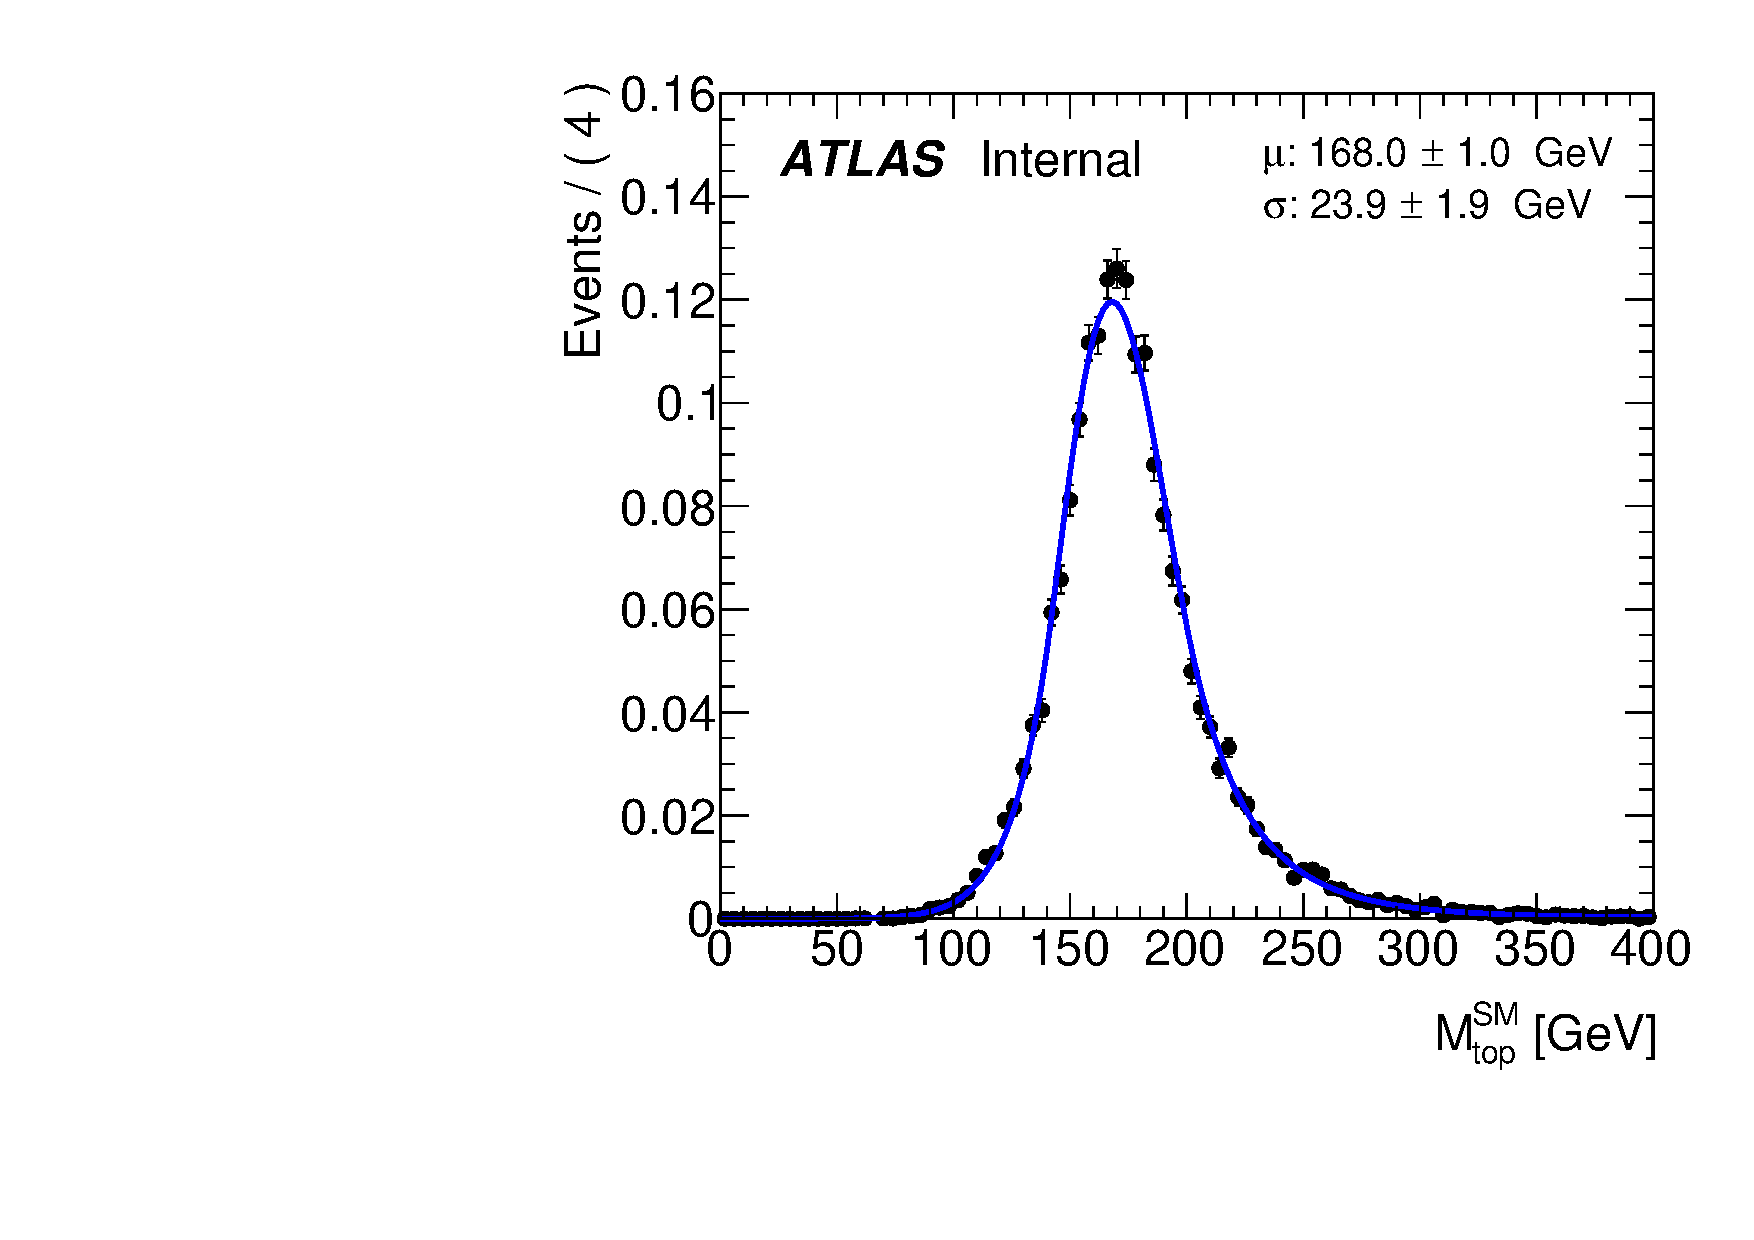
\includegraphics[width=.45\textwidth]{Appendices/AP2/figures/topSM} \\
				\multicolumn{2}{c}{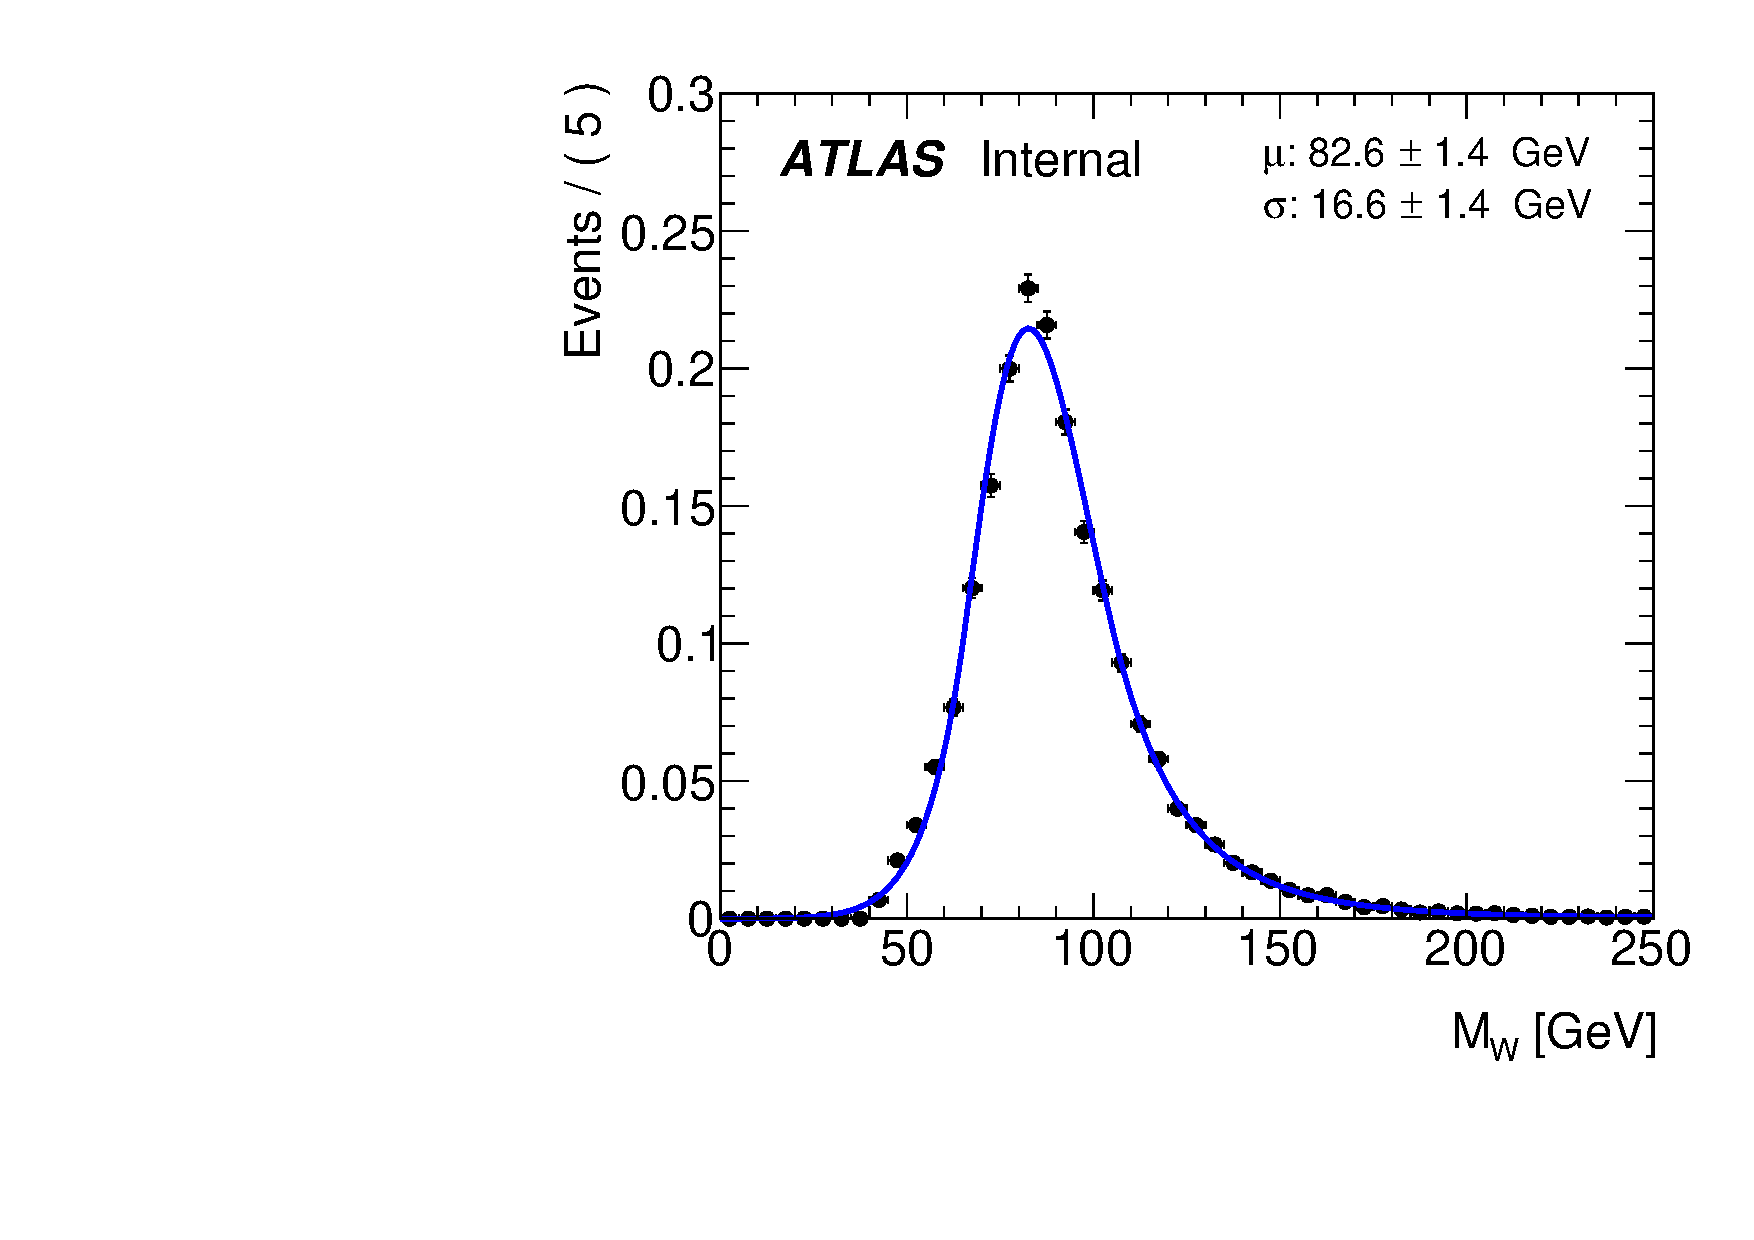
\includegraphics[width=.45\textwidth]{Appendices/AP2/figures/W}}
			\end{tabular}
			\caption{
			}%
			\label{fig:app-mass:bla}
%		\end{adjustwidth}
\end{figure}

%\sisetup{parse-numbers = false}
%\begin{table}[htbp]
%	\label{tab:mass-chi2}
%	\centering
%	\tiny
%	\begin{tabular}{l|cc|cc|cc}
%		\toprule
%		Region & \multicolumn{2}{c|}{FCNC top} & \multicolumn{2}{c|}{SM top} & \multicolumn{2}{c}{\PW} \\
%		& mass & $\sigma$ & mass & $\sigma$ & mass & $\sigma$ \\
%		\midrule
%		SR1 & \SI{171.1 \pm 1.6}{\GeV}  & \SI{11.4 \pm 1.4}{\GeV}  & \SI{167.2 \pm 3.6}{\GeV}  & \SI{22.5 \pm 2.6}{\GeV}  & \SI{82.8 \pm 1.6}{\GeV}  & \SI{16.1 \pm 1.4}{\GeV}  \\
%		SR2 & -- & --  & \SI{169.0 \pm 2.2}{\GeV}  & \SI{20.3 \pm 2.4}{\GeV}  & \SI{82.0 \pm 1.2}{\GeV}  & \SI{13.3 \pm 1.6}{\GeV}  \\
%		SR3 & \SI{158.1 \pm 1.2}{\GeV}  & \SI{11.9 \pm 1.5}{\GeV}  & \SI{165.5 \pm 1.5}{\GeV}  & \SI{27.0 \pm 1.7}{\GeV}  & \SI{82.8 \pm 1.8}{\GeV}  & \SI{17.8 \pm 1.6}{\GeV}  \\
%		\bottomrule
%	\end{tabular}
%\caption{
%	Summary of values of the mass and widths for the $\chi^2$ expressions. 
%}%
%\end{table}
%\restoregeometry


% ---------------------------------------------------------------------------
% ----------------------- end of thesis sub-document ------------------------
% ---------------------------------------------------------------------------

